\documentclass[tikz,margin=3.14mm, usenames, dvipsnames]{standalone}
\usepackage{tikz}
\usetikzlibrary{backgrounds}
\begin{document}

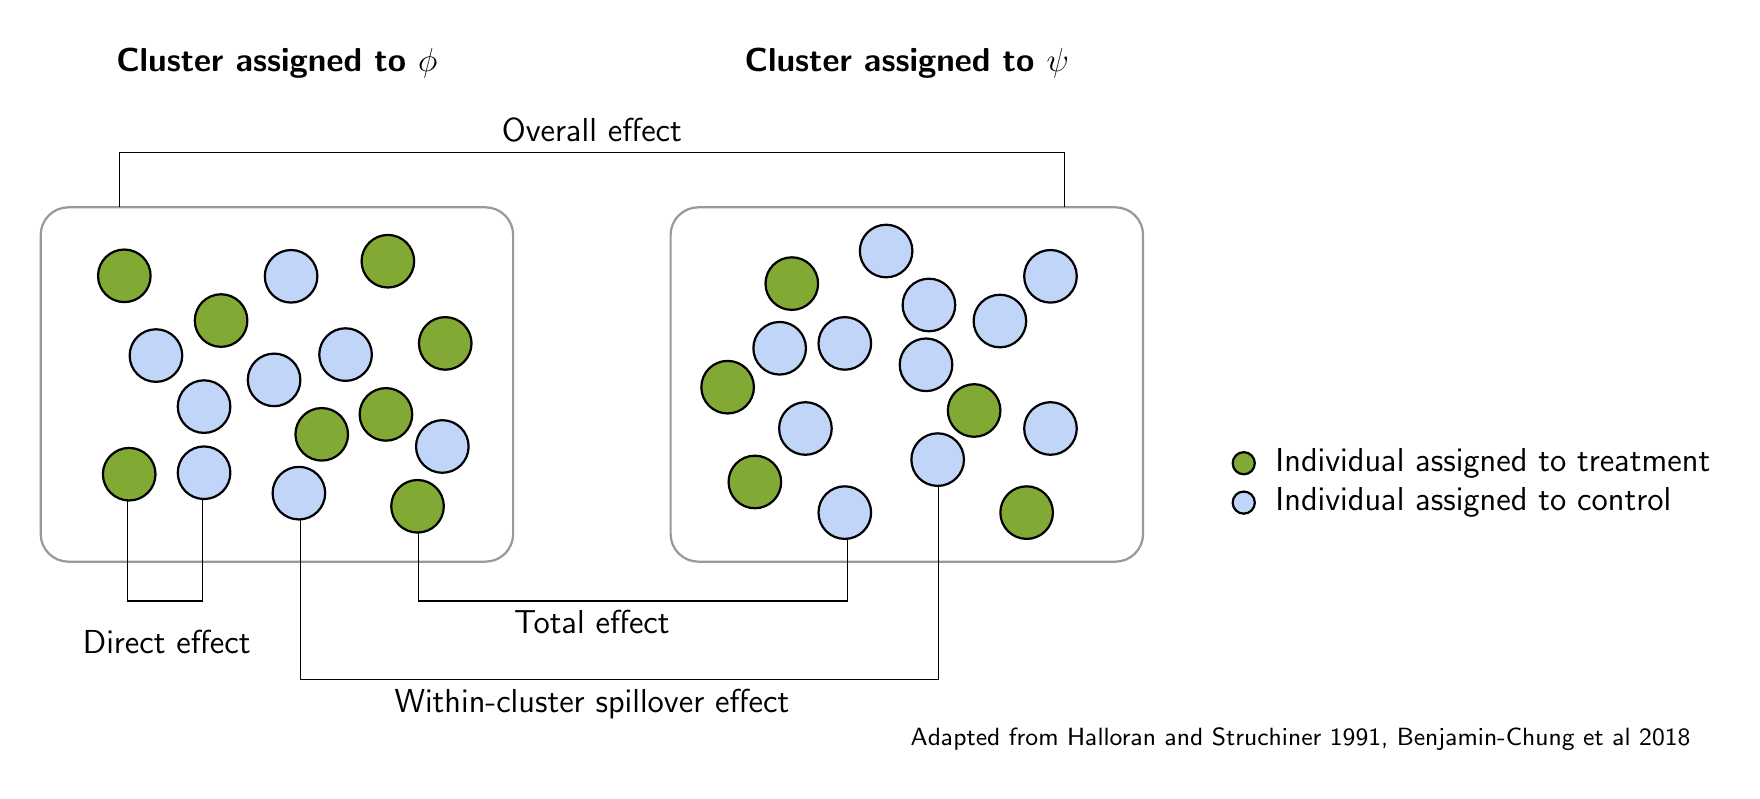
\begin{tikzpicture}[
    treated/.style={fill=YellowGreen!80!black!95, draw=black, thick},
    control/.style={fill=CornflowerBlue!40, draw=black, thick},
    font=\large\sffamily,
    background rectangle/.style={fill=white}, show background rectangle
    ]

    % Clusters
    \node[draw = black!40, thick, minimum width=6cm, minimum height=4.5cm, rounded corners=10, label={[label distance=1.5cm]above:\textbf{Cluster assigned to $\mathbf\phi$}}] (phi) at (0,0) {};
    \node[draw = black!40, thick, minimum width=6cm, minimum height=4.5cm, rounded corners=10, label={[label distance=1.5cm]above:\textbf{Cluster assigned to $\mathbf\psi$}}] (psi) at (8,0) {};

    % Coordinates transformation (scaling and shifting)
    \begin{scope}[shift={(phi.south west)},xscale=4.75,yscale=4.75]
        % Green dots in phi 
        \foreach \x/\y in {-0.018/0.744, 0.181/0.652, 0.524/0.774, 0.642/0.605, -0.008/0.336, 0.388/0.418, 0.520/0.459, 0.585/0.270} {
            \fill[treated] (\x*1.3+.25,\y*1.3-.2) circle (2pt);
        }
        % Blue dots in phi 
        \foreach \x/\y in {0.047/0.580, 0.325/0.743, 0.146/0.475, 0.290/0.530, 0.437/0.582, 0.341/0.297, 0.636/0.393, 0.146/0.339} {
            \fill[control, draw=black] (\x*1.3+.25,\y*1.3-.2) circle (2pt);
        }
    \end{scope}

    % Coordinates transformation for control
    \begin{scope}[shift={(psi.south west)-3},xscale=4.75,yscale=4.75]
        % Blue dots in psi 
        \foreach \x/\y in {1.290/0.728, 
          1.665/0.467, 1.773/0.257, 1.214/0.320,  1.158/0.515} {
            \fill[treated, draw=black] (\x*1.3-1.35,\y*1.3-.2) circle (2pt);
        }
        % Blue dots in psi 
        \foreach \x/\y in {1.484/0.795, 1.566/0.561, 1.265/0.595, 1.399/0.605,1.822/0.430, 1.572/0.684,  1.718/0.651,
          1.822/0.743,1.590/0.366,1.399/0.257,1.318/0.430} {
            \fill[control, draw=black] (\x*1.3-1.35,\y*1.3-.2) circle (2pt);
        }
    \end{scope}

    % Legend
    \node[anchor=west, label=right:Individual assigned to treatment] at (12, -1) {\tikz\fill[treated] (0,0) circle (4pt);};
    \node[anchor=west, label=right:Individual assigned to control] at (12, -1.5) {\tikz\fill[control] (0,0) circle (4pt);};

    % Labels for effects
    \node[below, align=center] (DE) at (-1.4,-3) {Direct effect};
    \node[below, align=center] (TE) at (4,-2.75) {Total effect}; 
    \node[below, align=center] (IE) at (4,-3.75) {Within-cluster spillover effect};
    \node[below] (OE) at (4,3.5) {Overall effect};

    \draw (-1.9,-1.45) |- (-.95,-2.75) -| (-.95, -1.45); % line for direct effect

    \def\TEx{1.8}
    \def\TExx{7.25}
    \def\TEy{-1.87}
    \def\TEyy{-1.95}
    \draw (\TEx,\TEy) |- (\TEx,-2.75) -| (\TExx, \TEyy);

    \def\IEx{0.3}
    \def\IExx{8.4}
    \def\IEy{-1.7}
    \def\IEyy{-1.28}
    \draw (\IEx,\IEy) |- (\IEx,-3.75) -| (\IExx, \IEyy);

    \def\OEx{-2}
    \def\OExx{10}
    \def\OEy{2.25}
    \def\OEyy{2.25}
    \draw (\OEx,\OEy) |- (\OEx,2.95) -| (\OExx, \OEyy);

    \node [align=left] at (13, -4.5) {\small Adapted from Halloran and Struchiner 1991, Benjamin-Chung et al 2018};
\end{tikzpicture}

\end{document}
